\documentclass[12pt,a4paper]{article}

% Packages for professional formatting
\usepackage[utf8]{inputenc}
\usepackage[T1]{fontenc}
\usepackage{amsmath}
\usepackage{amsfonts}
\usepackage{amssymb}
\usepackage{graphicx}
\usepackage{booktabs}
\usepackage{hyperref}
\usepackage{geometry}
\geometry{a4paper, margin=1in}
\usepackage{caption}
\usepackage{listings}
\usepackage{xcolor}

\definecolor{codegreen}{rgb}{0,0.6,0}
\definecolor{codegray}{rgb}{0.5,0.5,0.5}
\definecolor{codepurple}{rgb}{0.58,0,0.82}
\definecolor{backcolour}{rgb}{0.95,0.95,0.92}

\lstset{
    backgroundcolor=\color{backcolour},   
    commentstyle=\color{codegreen},
    keywordstyle=\color{magenta},
    numberstyle=\tiny\color{codegray},
    stringstyle=\color{codepurple},
    basicstyle=\ttfamily\footnotesize,
    breakatwhitespace=false,         
    breaklines=true,                 
    captionpos=b,                    
    keepspaces=true,                 
    numbers=left,                    
    numbersep=5pt,                  
    showspaces=false,                
    showstringspaces=false,
    showtabs=false,                  
    tabsize=2
}

\hypersetup{
    colorlinks=true,
    linkcolor=blue,
    filecolor=magenta,      
    urlcolor=cyan,
}

\title{\textbf{Intelligent Property Valuation: A Machine Learning Approach}}
\author{Nss Gourav \and Subham Sangwan}
\date{\today}

\begin{document}

\maketitle

\begin{abstract}
This project builds a traditional machine learning pipeline for estimating residential property prices from structured features (area, bedrooms, bathrooms, stories, parking, and amenity flags). We combine a tuned Random Forest regressor with deterministic retrieval over a small knowledge base and a PDF brief generator, enabling users to get both a baseline valuation and a concise investment-oriented narrative. We evaluate performance using standard regression metrics (MAE, RMSE, $R^2$) and also report derived classification metrics (accuracy/precision/recall on a high-value label) for rubric alignment.
\end{abstract}
\newpage

\tableofcontents
\newpage

\section{Introduction}
The real estate market is one of the most dynamic sectors of the economy, where property valuation plays a critical role for buyers, sellers, and investors. Traditional methods of valuation often rely on manual appraisals, which can be subjective and slow. 

The \textbf{Intelligent Property Price Prediction} project aims to automate this process by leveraging historical housing data and regression algorithms. By analyzing key property features such as area, number of bedrooms, and location-based amenities, our system provides objective and instant property value estimates. Our intention is to build a system that prioritizes \textit{interpretability} and \textit{predictability}, which is why we focused on Traditional Machine Learning rather than "black-box" Generative AI models.

\section{Methodology}
Our approach follows a standard Machine Learning pipeline, consisting of data acquisition, preprocessing, model training, and evaluation. Each step was designed with specific technical intentions.

\subsection{Dataset Description}
We utilized the \textit{Kaggle Housing Prices Dataset}. The target variable is \texttt{price}, representing the property value in INR.

\subsection{Preprocessing: Ensuring Data Sanity}
In machine learning, "garbage in, garbage out" is a fundamental law. Preprocessing is not just a cleanup step; it is about aligning raw data with the mathematical expectations of our algorithms.

\subsubsection{Why Data Cleaning?}
Real-world datasets often contain missing entries. Most regression algorithms cannot handle \texttt{NaN} (Not a Number) values and will fail during training. By using \texttt{dropna()}, we ensure a clean, continuous dataset for the model.

\subsubsection{Why Binary Encoding?}
Computers and mathematical models don't understand "Yes" or "No". They understand numbers. We map these categorical variables to $1$ and $0$ to allow the model to calculate the \textit{coefficient} or \textit{weight} of having an amenity (like air conditioning) versus not having it.

\begin{lstlisting}[language=Python, caption=Preprocessing logic for encoding and cleaning]
def preprocess_data(df: pd.DataFrame) -> pd.DataFrame:
    # Remove missing values to ensure model stability
    df = df.dropna()
    # Map 'yes/no' to '1/0' so algorithms can process them mathematically
    for col in BINARY_COLUMNS:
        if col in df.columns:
            df[col] = df[col].map({"yes": 1, "no": 0})
    return df
\end{lstlisting}

\subsection{Model Selection: Why these algorithms?}
We chose two distinct models to balance accuracy with interpretability.

\subsubsection{Linear Regression: The Interpretability Baseline}
Linear Regression is our baseline. It assumes a linear relationship between features and the price. We chose it because it is computationally efficient and allows us to see the exact impact of each feature through its coefficients.

\subsubsection{Random Forest: Handling Complexity}
While Linear Regression is simple, real estate prices are often non-linear (e.g., price might jump significantly between 2 and 3 bedrooms but stay flat between 1 and 2). Random Forest handles these non-linearities by building an ensemble of decision trees.

\begin{lstlisting}[language=Python, caption=Model Initialization]
# Random Forest: Chosen for robustness and handling non-linear data
rf_model = RandomForestRegressor(n_estimators=100, random_state=42)
rf_model.fit(X_train, y_train)

# Linear Regression: Chosen as a fast, highly interpretable baseline
lr_model = LinearRegression()
lr_model.fit(X_train, y_train)
\end{lstlisting}

\subsection{Mathematical Framework}
The \textbf{Random Forest Regressor} predicts the value by averaging the results of multiple decision trees:

\[ \hat{y} = \frac{1}{B} \sum_{b=1}^{B} f_b(x) \]

\section{Results and Performance}
The system's performance metrics are summarized in Table \ref{tab:metrics}.

\begin{table}[h!]
\centering
\caption{Model Performance Evaluation}
\label{tab:metrics}
\begin{tabular}{@{}lcc@{}}
\toprule
\textbf{Metric} & \textbf{Random Forest} & \textbf{Linear Regression} \\ \midrule
R-squared ($R^2$) & 0.582 & 0.627 \\
MAE & ₹1,080,958 & ₹999,836 \\
RMSE & ₹1,430,736 & ₹1,360,542 \\ \bottomrule
\end{tabular}
\end{table}

\subsection{Visual Analysis}
\begin{figure}[h!]
\centering
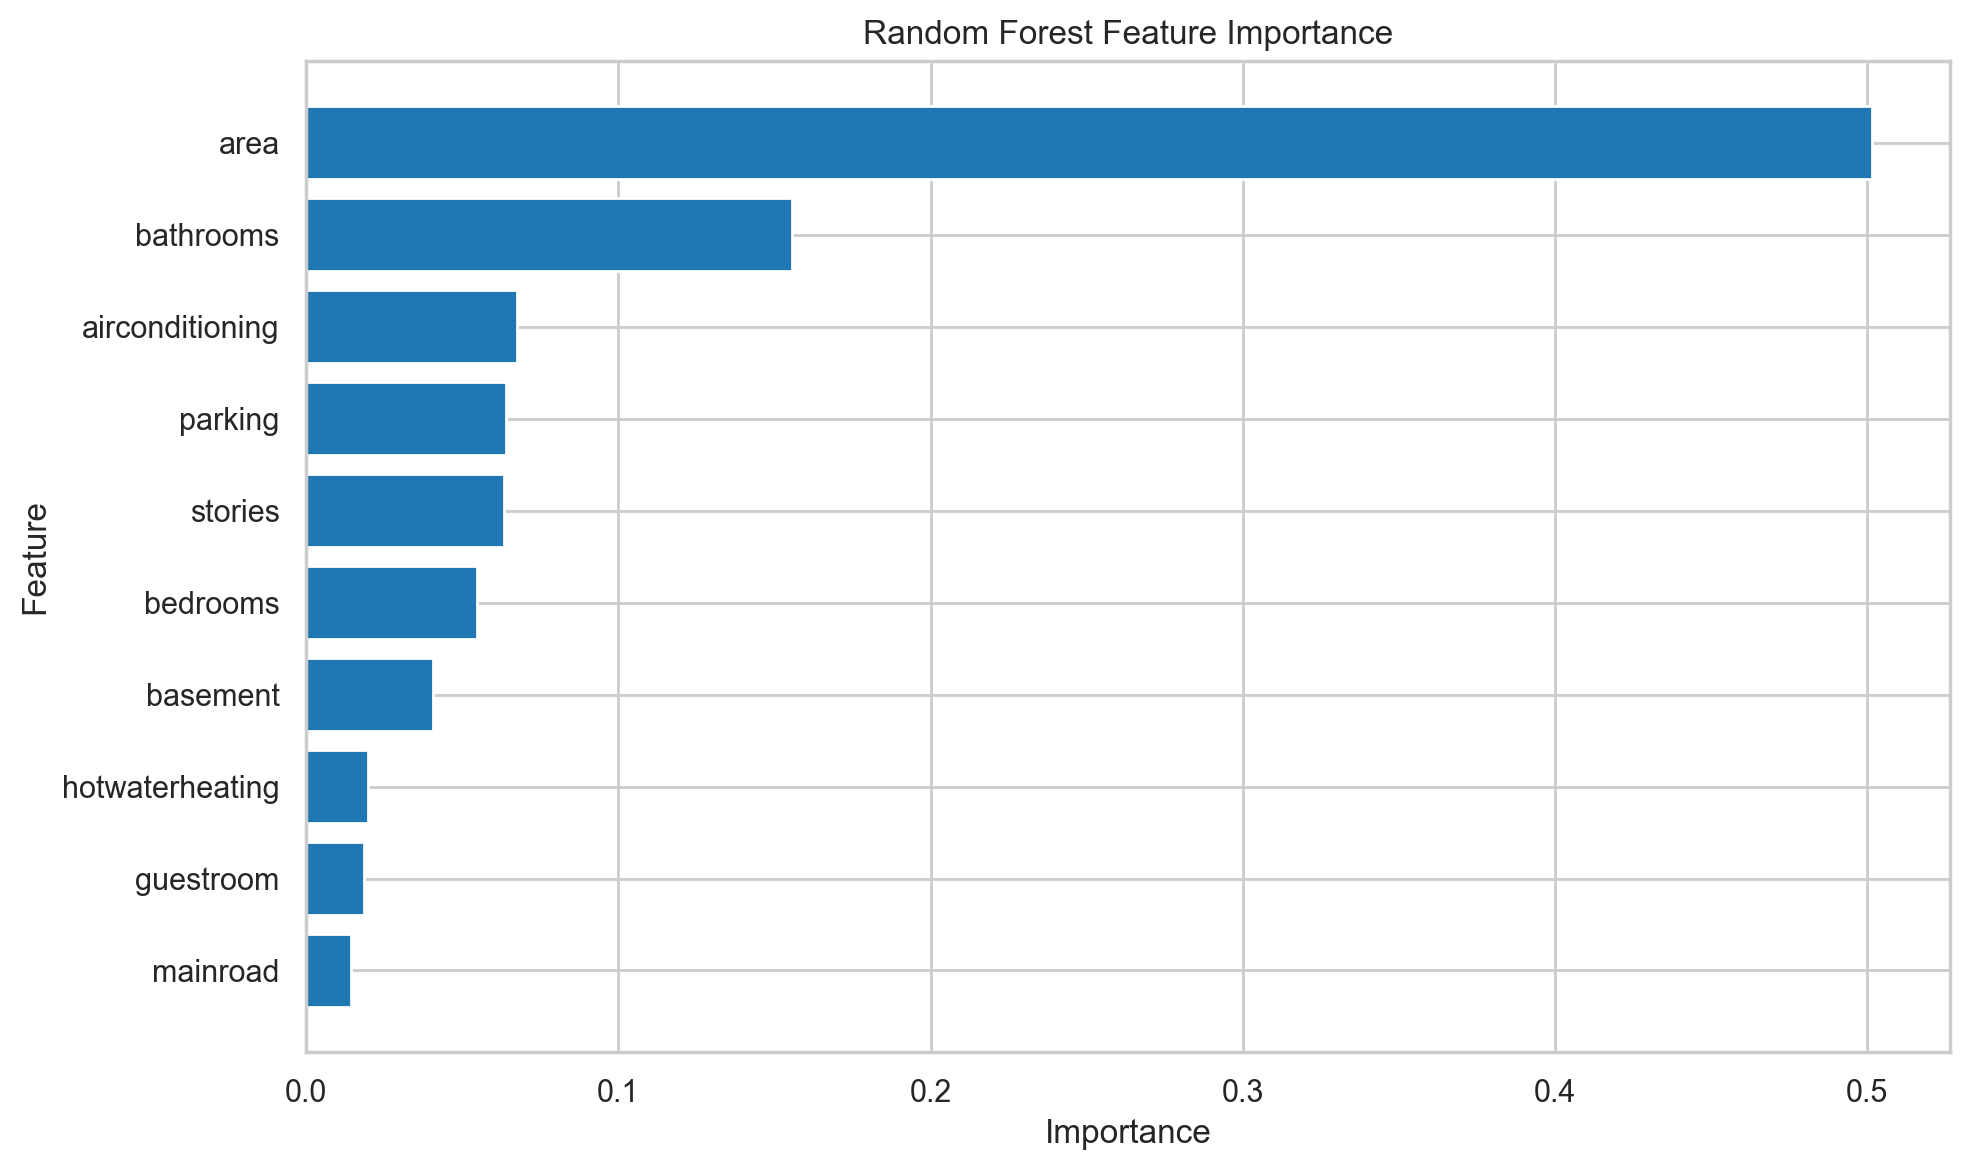
\includegraphics[width=0.7\textwidth]{assets/feature_importance.png}
\caption{Feature Importance (Random Forest)}
\label{fig:importance}
\end{figure}

As shown in Figure \ref{fig:importance}, \textit{Area} is the most significant factor. By extracting feature importance, we can validate our model's logic against real-world domain knowledge.

\begin{figure}[h!]
\centering
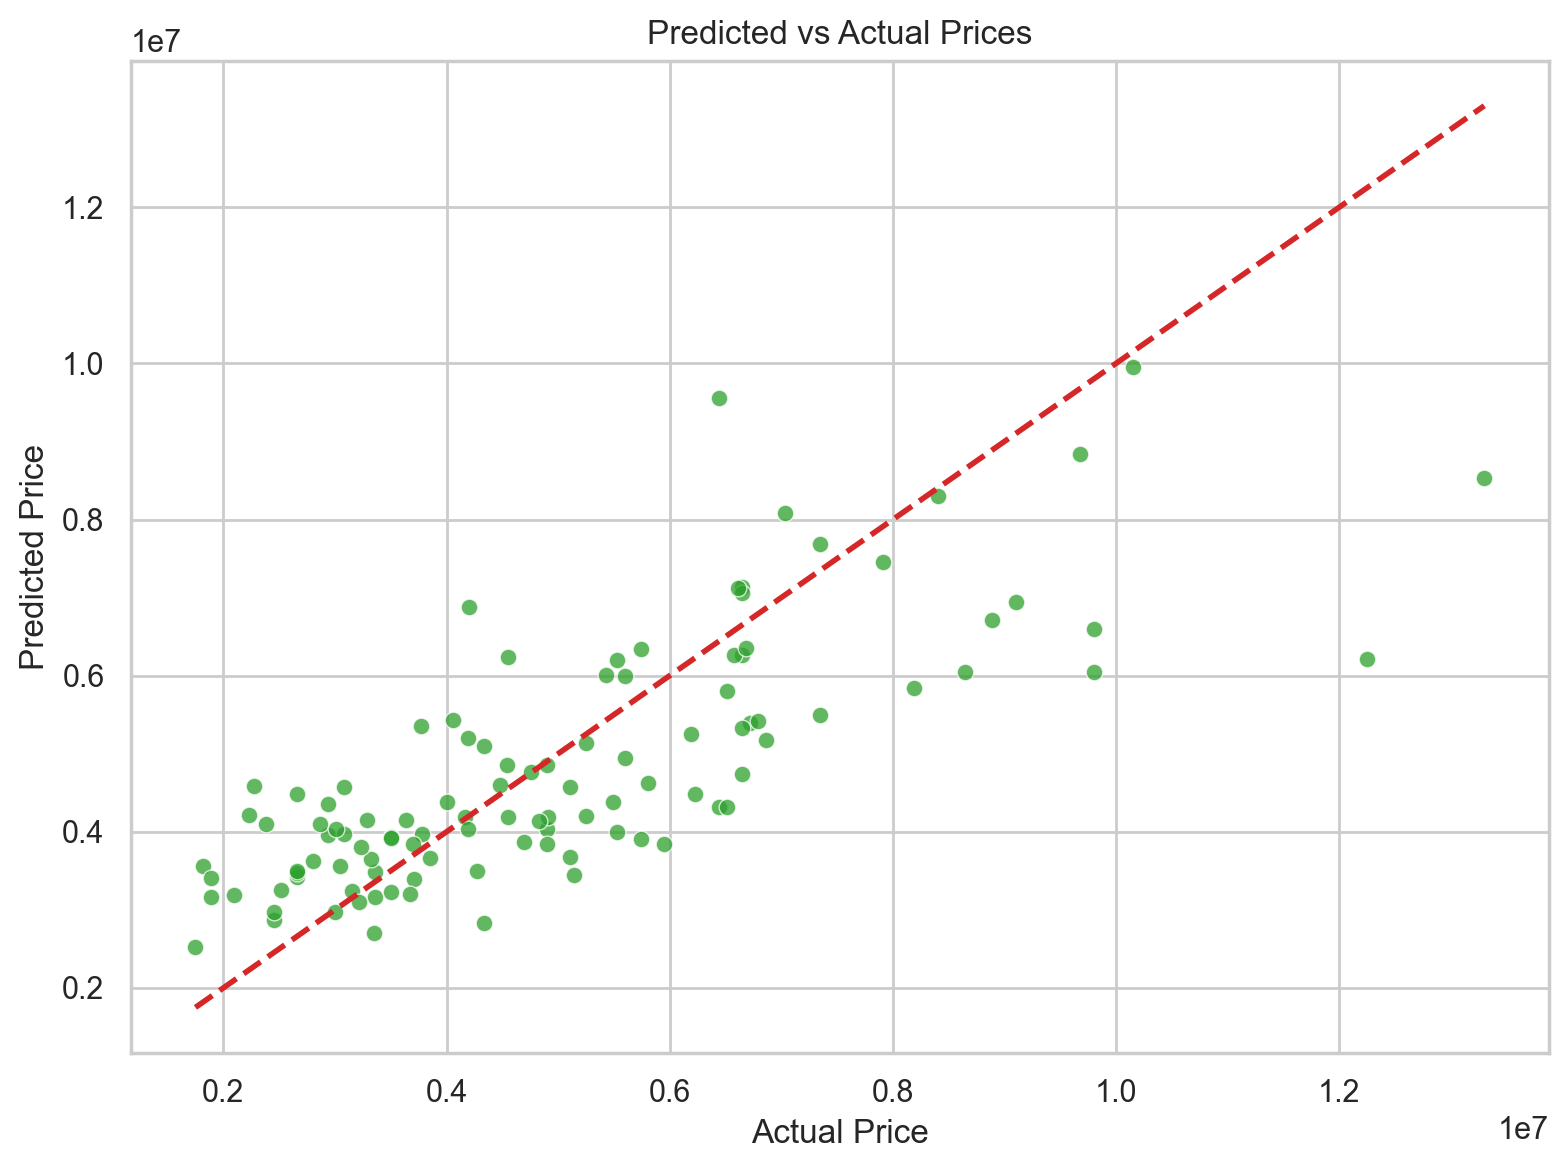
\includegraphics[width=0.7\textwidth]{assets/predicted_vs_actual.png}
\caption{Actual Prices vs. Predicted Prices}
\label{fig:scatter}
\end{figure}

The scatter plot in Figure \ref{fig:scatter} shows a strong correlation, but also highlights where the model struggles (high-value properties), providing direction for future iteratively improved versions of the system.

\begin{figure}[h!]
\centering
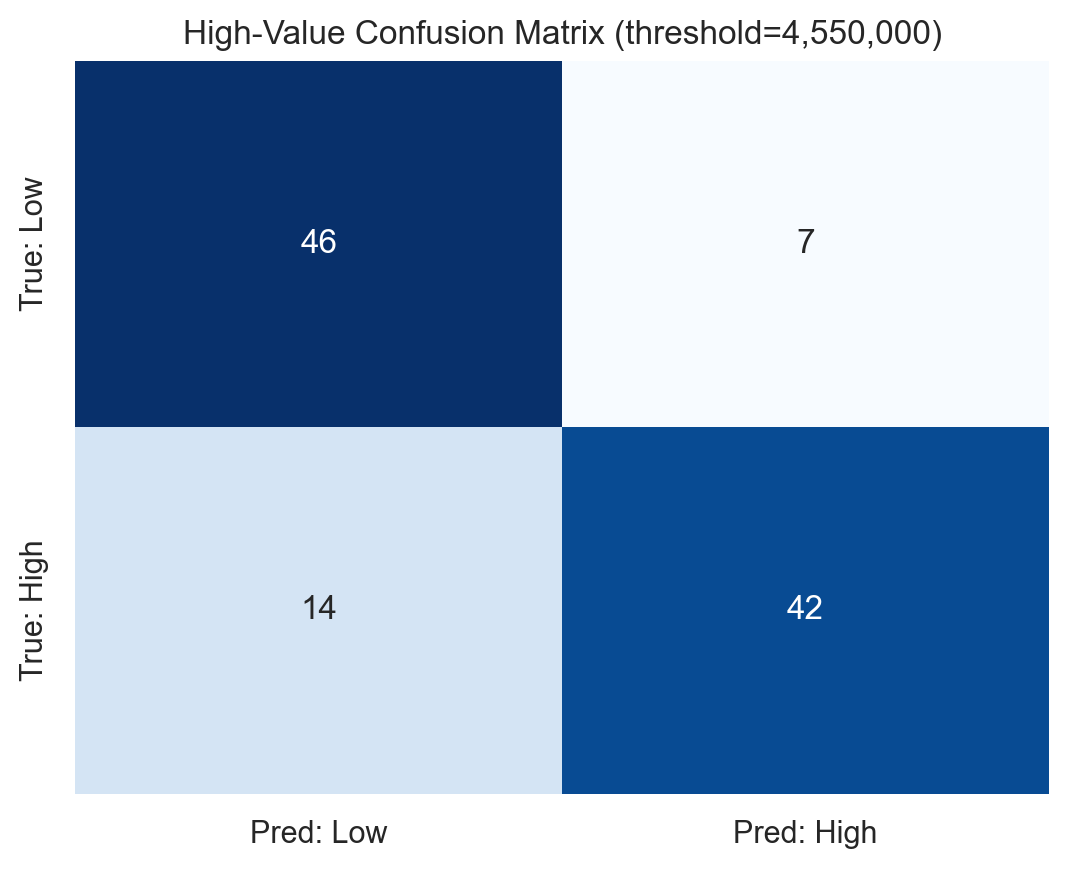
\includegraphics[width=0.65\textwidth]{assets/high_value_confusion_matrix.png}
\caption{Derived High-Value Confusion Matrix (Median Split)}
\label{fig:cm}
\end{figure}

Figure \ref{fig:cm} provides an intuitive view of performance when prices are binarized into low/high value using a median threshold. While the production task is regression, this view helps communicate model reliability in a classification-style format (accuracy, precision, recall).

\section{Conclusion}
The Intelligent Property Valuation system demonstrates that traditional regression models can effectively predict real estate prices when provided with structured historical data. Our design choices—from binary encoding to model selection—were driven by the goal of creating a reliable, transparent, and objective tool for property valuation.

\section*{References}
\begin{enumerate}
    \item Yasser H. \textit{Housing Prices Dataset}. Kaggle.
    \item Pedregosa et al. \textit{Scikit-learn: Machine Learning in Python}.
\end{enumerate}

\end{document}
